\documentclass[french, a4paper, 12pt, titlepage]{article}
%% Peut remplacer "article" par "scrartcl" %%

\usepackage{a4wide}
%\usepackage[top=2cm, bottom=2cm, left=2cm, right=2cm]{geometry}
\raggedbottom % prevents vertical white space on pages that cannot be filled properly

\usepackage{hyperref}
\hypersetup{
	colorlinks=true,       	% false: boxed links; true: colored links
	linkcolor=black,          	% color of internal links
	urlcolor=blue,           	% color of external links
	citecolor=grey
}

\usepackage[T1]{fontenc}
%\usepackage{fourier}
%\usepackage{utopia}
%\usepackage{palatino}

\usepackage{lmodern}
%% ajouter fonte petite capitale grasse à lmodern avec celle de computer modern %%
\rmfamily
\DeclareFontShape{T1}{lmr}{b}{sc}{<->ssub*cmr/bx/sc}{}
\DeclareFontShape{T1}{lmr}{bx}{sc}{<->ssub*cmr/bx/sc}{}
%% /ajout %%
\usepackage{wrapfig}

%\usepackage[a4paper]{geometry} % marges plus petites que a4paper standard
\usepackage{listings} % insérer code source
%\usepackage{algorithm} % algorithmique
%\usepackage{algorithmic}
\usepackage{url}
\usepackage[usenames, dvipsnames]{color} % couleurs (nombre de base étendu)
\usepackage{graphicx} % insérer images
\usepackage[utf8]{inputenc}
\usepackage[french]{babel}
\usepackage{amsmath}
\usepackage{amsfonts}
\usepackage{amssymb}
\usepackage{amsthm}
\usepackage{multicol}
\definecolor{grey}{rgb}{0.96,0.96,0.96}
\definecolor{grey2}{rgb}{0.3,0.3,0.3}

%% Define listings params %%
\lstset{
	numbers=left,
	language=Java,
	tabsize=4,
	frame=single, % cadre autour du code
	breaklines=true, % autorise couper ligne trop longue
	basicstyle=\small\ttfamily,
	numberstyle=\scriptsize\ttfamily,
	backgroundcolor=\color{grey},
	showstringspaces=false,
	keywordstyle=\color{OliveGreen},
	stringstyle=\color{BrickRed},
	commentstyle=\color{grey2}\it,
	stepnumber=1
} % numérote toute les x lignes
% listing utf8 fr %
\lstset{%
	inputencoding=utf8,
	extendedchars=true,
	literate=
		{é}{{\'{e}}}1
		{è}{{\`{e}}}1
		{ê}{{\^{e}}}1
		{ë}{{\¨{e}}}1
		{û}{{\^{u}}}1
		{ù}{{\`{u}}}1
		{â}{{\^{a}}}1
		{à}{{\`{a}}}1
		{î}{{\^{i}}}1
		{ç}{{\c{c}}}1
		{Ç}{{\c{C}}}1
		{É}{{\'{E}}}1
		{Ê}{{\^{E}}}1
		{À}{{\`{A}}}1
		{Â}{{\^{A}}}1
		{Î}{{\^{I}}}1
}
%% /Define listings params %%

%% Francisation des algorithmes
%\renewcommand{\algorithmicrequire} {\textbf{\textsc{Entrées:}}}
%\renewcommand{\algorithmicensure}  {\textbf{\textsc{Sorties:}}}
%\renewcommand{\algorithmicwhile}   {\textbf{tant que}}
%\renewcommand{\algorithmicdo}      {\textbf{faire}}
%\renewcommand{\algorithmicendwhile}{\textbf{fin tant que}}
%\renewcommand{\algorithmicend}     {\textbf{fin}}
%\renewcommand{\algorithmicif}      {\textbf{si}}
%\renewcommand{\algorithmicendif}   {\textbf{fin si}}
%\renewcommand{\algorithmicelse}    {\textbf{sinon}}
%\renewcommand{\algorithmicthen}    {\textbf{alors}}
%\renewcommand{\algorithmicfor}     {\textbf{pour}}
%\renewcommand{\algorithmicforall}  {\textbf{pour tout}}
%\renewcommand{\algorithmicdo}      {\textbf{faire}}
%\renewcommand{\algorithmicendfor}  {\textbf{fin pour}}
%\renewcommand{\algorithmicloop}    {\textbf{boucler}}
%\renewcommand{\algorithmicendloop} {\textbf{fin boucle}}
%\renewcommand{\algorithmicrepeat}  {\textbf{répéter}}
%\renewcommand{\algorithmicuntil}   {\textbf{jusqu'à}}
%\renewcommand{\algorithmiccomment} {\STATE //}
%\newcommand{\BEGIN}{\STATE \fbox{Début}}
%\newcommand{\END}{\STATE \fbox{Fin}}
%\floatname{algorithm}{Algorithme}
%% /francisation des algorithmes

\renewcommand{\qedsymbol}{}

\newcommand{\petit}[1]{
	\medskip \noindent
	\begin{small}
	#1)
	\end{small}
}

\newcommand{\graph}[2]{
\medskip
	\begin{center}
		\includegraphics[scale=#1]{#2}
	\end{center}
\medskip
}

\begin{document}

\title{Atelier Systèmes d'Exploitation\\Simulation Interbancaire}
\author{\textsc{Martel} Damien}
\date{Compilé le \today}

\maketitle
%% Laisse page blanche pour verso page de garde %%

\vfill
\pagebreak

%\tableofcontents
\newpage
\strut\thispagestyle{empty}
\vfill
\pagebreak
\tableofcontents
\strut\thispagestyle{empty}
%\setcounter{page}{0}
\newpage
\setcounter{page}{1}

\section{Schéma général de la simulation}
\medskip
\begin{center}
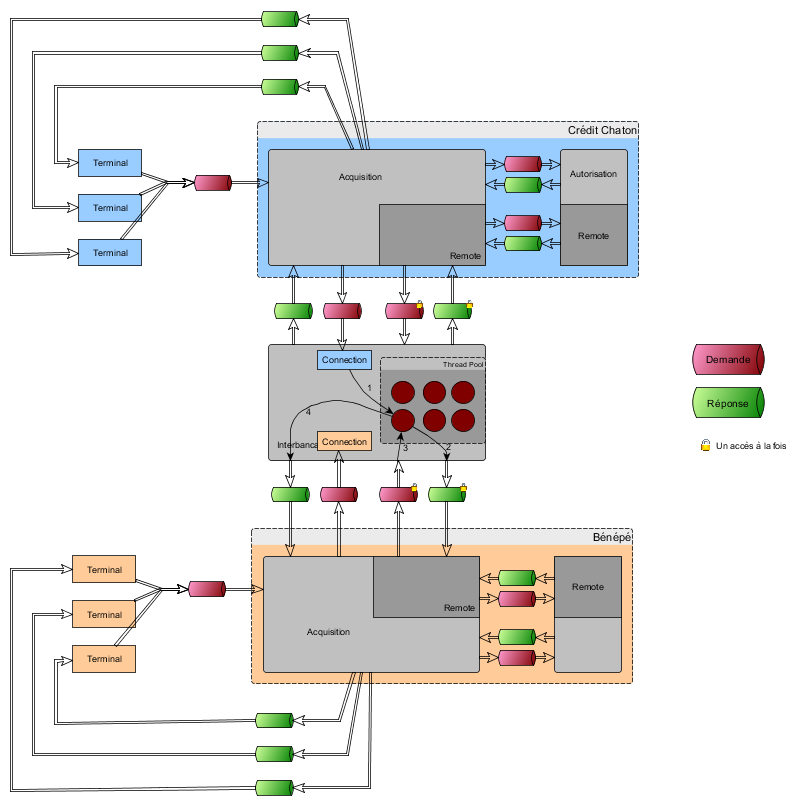
\includegraphics[scale=0.5]{global}
\end{center}
\medskip

Tout au long de ce manuel, nous utiliserons la notion de connexion locale et distante.
Une connexion locale signifie qu'un terminal associé à une banque émet une demande pour un débit sur un compte de cette même banque (terminal crédit chaton utilisé par un client de crédit chaton), alors qu'une connexion distante se réfère à un client utilisant un terminal associé à une autre banque (client de la bénépé utilisant un terminal de crédit chaton).
Ces deux cas traités par le même serveur d'acquisition sont routés différemment et passent par deux parties différentes de l'application.

\section{Serveurs mis en place}
Pour cette simulation, un minimum de 3 serveurs est nécessaire afin d'effectuer des transactions locales
(un client utilisant un terminal de sa banque),
2 serveurs supplémentaires par client de banque différents pour les transactions à distance (un client utilisant le terminal d'une autre banque que la sienne).

Les 3 serveurs permettant les connexions locales sont les suivantes:

\begin{itemize}
\item Terminal
\item Acquisition
\item Autorisation
\end{itemize}

Afin de permettre un connexion distante, il faut rajouter pour cela le serveur Interbancaire, connecté à un autre couple de serveur Acquisition/Autorisation associé à une banque.

\section{Déroulement d'une transaction}
\subsection{Local}
En utilisant un terminal de sa propre banque, une demande est effectuée au serveur d'acquisition qui retransmettra l'information au serveur d'autorisation.
Une fois cette demande traitée, le serveur d'autorisation renverra au serveur d'acquisition la réponse qui pourra signaler au terminal, à l'aide d'un tube dédié.
\medskip
\begin{center}
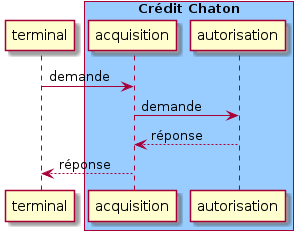
\includegraphics[scale=0.7]{transactionLocal}
\end{center}
\medskip

\subsection{Distante}
Pour l'utilisation d'un terminal d'une autre banque, le chemin est légèrement plus long.
Le serveur d'acquisition, qui récupère une demande avec un identifiant de banque différent du sien, enverra la demande au serveur interbancaire à travers un tube qui lui est propre.\\
\noindent
Le serveur interbancaire possède pour chaque tube relié à une banque, un thread s'occupant d'encapsuler la demande en y rajoutant, la banque émettant la demande, la banque à laquelle est destinée cette demande ainsi que la demande en elle même avant de l'envoyer à travers un tube relié à la partie centrale du serveur s'occupant de router ces demandes, d'en attendre la réponse et la renvoyer à la bonne banque.
Cette partie est implémentée sous la forme d'une piscine de processus léger (thread pool) dont le nombre limite la quantité de demandes simultanées qu'elle peut traiter.\\
\noindent
Les serveurs d'acquisition disposent ainsi d'un deuxième chemin d'accès à u serveur d'autorisation différenciant les demandes émises par un terminal associé à une banque ou provenant du serveur interbancaire, leur permettant de renvoyer des réponses distantes au serveur interbancaire.
\medskip
\begin{center}
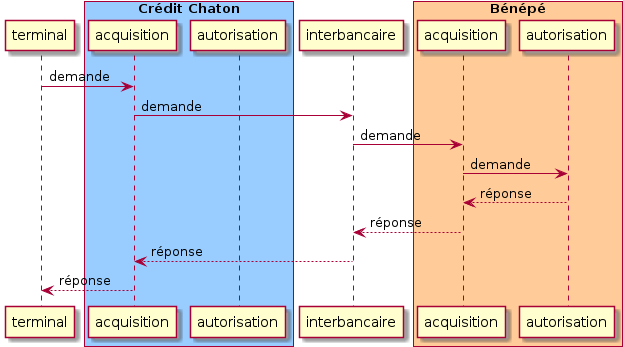
\includegraphics[scale=0.6]{transactionDistante}
\end{center}
\medskip

\section{Arbre des processus}
\graph{0.6}{arbre}
Chaque serveur se lance de manière indépendante, et n'ont pas de lien de parenté direct, ils utilisent donc pour communiquer des tubes nommés en respectant une certaine convention de nommage.\\
\noindent
Afin de pouvoir lancer chaque processus dans l'ordre que l'on veut, ils essayeront tous de créer le tube afin d'éviter des erreurs de l'ordre de \og No such file or directory \fg\\
\noindent
Enfin, si les processus doivent effectuer plusieurs actions de manière asynchrone, ils créeront des threads dont le nombre ne sera limité que si nécessaire,
c'est-à-dire que dans une logique de parallélisation, la création de plus de threads sert à exécuter la même action (comme dans le serveur interbancaire) au lieu d'effectuer une autre action légèrement différente (comme dans le serveur d'acquisition).\\
\noindent
Ainsi le parallélisme n'est pas obtenu en augmentant un paramètre déterminant la quantité de ressource allouée au processus (nombre de thread) mais à l'exécution d'un nouveau serveur.\\
\noindent
Sauf pour le serveur Interbancaire, goulot d'étranglement des messages qui ne dispose pas à ce jour de design lui permettant cela.


\section{Communication}
Afin de pouvoir communiquer ensemble, et ne possédant pas de lien filial, les différents serveurs communiquent à l'aide de tubes nommées, et pour garantir leur communication, une certaine convention a été utilisée.\\
\noindent
Nous présenterons ici les chemins utilisés pour les différents tubes, afin de pouvoir différencier les différents serveurs associés aux banques, on peut parfois retrouver dans le nom un mot entre chevrons (\og <id> \fg) ceci signifie que le serveur doit le remplacer par la donnée correspondante (par exemple: <bankId> signifie que le serveur doit remplacer dans le nom du tube par l' identifiant de sa banque associée).

\subsection{Terminal}
Ce serveur est connecté à un tube en écriture et un autre en lecture.
\begin{description}
	\item[resources/bank<bankId>/input.fifo] (write) permet d'envoyer les demande à son serveur d'acquisition
	\item[resources/bank<bankId>/<cardNumber>.fifo] (write) permet de recevoir la réponse du serveur d'acquisition
\end{description}
\noindent
(ici <cardNumber> signifie que le tube doit être nommé à l'aide du numéro de carte qui émet la demande)
\graph{0.5}{terminal}
\subsection{Autorisation}
Ce serveur est connecté à deux tubes en écriture et deux tubes en lecture.
\begin{description}
	\item[resources/bank<bankId>/localAuth.fifo] (read) permet de recevoir des demande d'autorisation du serveur d'acquisition
	\item[resources/bank<bankId>/remoteAuthDemande.fifo] (read) permet de recevoir des demandes venant du serveur interbancaire
	\item[resources/bank<bankId>/response.fifo] (write) permet d'envoyer les réponses au serveur d'acquisition
	\item[resources/bank<bankId>/remoteInput.fifo] (write) permet d'envoyer des réponses au serveur interbancaire
\end{description}
\graph{0.5}{autorisation}
\subsection{Acquisition}
Ce serveur est connecté à 2 tubes en lecture et 5 tubes en écriture.
\begin{description}
	\item[resources/bank<bankId>/input.fifo] (read) permet de recevoir des demandes locales à traiter
	\item[resources/bank<bankId>/response.fifo] (read) permet de recevoir réponses locales à traiter
	\item[resources/bank<bankId>/remoteInput.fifo] (read) permet de recevoir des demandes ou des réponses distantes à traiter
	\item[resources/bank<bankId>/localAuth.fifo] (write) permet d'envoyer des demandes d'autorisation locales
	\item[resources/bank<bankId>/interRemoteDemande.fifo] (write) permet d'envoyer des demandes d'autorisation au serveur interbancaire
	\item[resources/bank<bankId>/<cardNumber>.fifo] (write) permet d'envoyer une réponse au terminal associé
	\item[resources/bank<bankId>/remoteAuthDemande.fifo] (write) permet d'envoyer une demande d'autorisation en provenance du serveur interbancaire
	\item[resources/bank<bankId>/interRéponse.fifo] (write) permet de renvoyer une réponse du serveur d'autorisation vers le serveur interbancaire
\end{description}
\graph{0.5}{acquisition}

\subsection{Interbancaire}
Pour ce serveur, le nombre de tubes auxquels il est connecté est dépendant du nombre de banques qu'il connecte.
Ainsi pour n banques reliées, il gère 4n tubes en lecture et 2n tubes en écriture, il possède aussi un tube interne dépendant de son implémentation (ne servant donc pas à communiquer avec les autres serveurs), que nous verrons dans une autre partie de ce manuel.

\begin{description}
	\item[resources/bank<bankId>/interRemoteDemande.fifo] (read) permet de recevoir des demandes d'autorisation d'une banque
	\item[resources/bank<bankId>/remoteInput.fifo] (read) permet de recevoir des demandes ou des réponses distantes à traiter
	\item[resources/bank<bankId>/interRéponse.fifo] (read) permet de recevoir une réponse d'un serveur d'autorisation d'une banque
	\item[resources/bank<bankId>/response.fifo] (write) permet d'envoyer des réponses distantes à une banque
\end{description}
\graph{0.5}{interbancaire}

\section{Fonctionnement des serveurs}
\subsection{Terminal}
Le terminal après avoir reçu une requête directement de l'entrée standard (stdin) qui correspond au numéro de carte du client, envoie une demande au serveur d'acquisition puis attend une réponse de ce même serveur avant de recommencer.
\graph{0.4}{terminalState}

\subsection{Autorisation}
Le serveur d'autorisation est découpé en deux parties exécutant la même fonction ayant pour différence la paire de tubes connectée à ces threads.
Ils reçoivent tous deux une demande sur leur tube ouvert en lecture pour vérifier dans leur annuaire la validité de la transaction, puis renvoient une réponse sur les tubes ouverts en écriture correspondants.
L'annuaire est mis en mémoire depuis un fichier contenant un numéro de carte bancaire suivi de la somme disponible sur le compte et ce pour chaque ligne du fichier.
Cet annuaire est formé par une structure contenant la taille de cette structure (correspondant au nombre de lignes du fichier chargé) et d'un tableau flexible de chaînes de caractères.
\graph{0.4}{autorisationState}

\subsection{Acquisition}
Ce serveur est connecté à tous les autres et possède lui aussi deux parties.
La première s'occupant des messages distants, ne fait que relayer les messages entre le serveur d'autorisation et le serveur interbancaire.
\graph{0.5}{acquisitionStateRemote}
La deuxième partie s'occupe des demande locales. Elle reçoit dans son unique point d'entrée à la fois les demandes émises par les terminaux et les réponses du serveur d'autorisation.
Les réponses sont directement retransmises aux terminaux, alors que les demandes sont envoyées, soit au serveur d'autorisation si leur code bancaire correspond à son numéro de banque, alors que les autres sont retransmises au serveur interbancaire.
\graph{0.4}{acquisitionStateLocal}

\subsection{Interbancaire}
Le serveur interbancaire doit gérer les messages distants, une demande émise par une banque à l'attention d'un serveur d'autorisation distant.
Pour cela, le serveur interbancaire crée une \og connexion\fg{}, c'est-à-dire un thread associé à une série de tubes, par banque.
Ce thread permet de différencier et retenir le chemin de chaque demande pour pouvoir renvoyer la réponse au bon endroit.
En plus de chaque connexion, et pour pouvoir gérer simultanément une multitude de messages, le serveur interbancaire crée une piscine de processus léger (thread pool)
permettant de stocker la route de retour et d'attendre le message d'autorisation distant.
Cette quantité de threads créée correspond au nombre de messages que peut traiter simultanément. \\

Chacun de ces threads de travail sont connectés à un tube servant à distribuer chaque demande au premier processus libre.
Les différentes connexions encapsulent la demande en indiquant les informations essentielles (message à transmettre, banque destinataire et banque de retour).
Une fois un message reçu par les threads de travail, le message est envoyé puis une réponse est attendue avant de pouvoir la renvoyer.
Pour l'instant n'ayant pas implémenté un design plus souple et hautement plus compliqué, et afin que les réponses soient reçues par les threads les attendant, chacun d'eux va verrouiller l'accès au tube de réponse distant associé à la banque à laquelle ils envoient leur demande.

\graph{0.4}{piscine}


\subsubsection{Design plus souple et hautement plus compliqué}
La solution pensée pour permettre à chaque thread de pouvoir recevoir la demande qu'ils attendent serait de simplement broadcaster toutes les réponses à tous les threads, c'est-à-dire créer un deuxième tube reliant chacun des threads à une sous routine \og broadcast\fg{} servant à copier les réponses à un tube dédié sur les processus de travail.
En plus de cela, chacun des threads devra pour ne pas bloquer le broadcast, continuellement lire ce tube afin de rejeter les réponses qu'ils n'attendent pas, en fonction d'un filtre mis en place avant l'envoi d'une demande.\\
\noindent
Il se pose alors un problème de scalabilité, afin de pouvoir simplement augmenter les performances en lançant un deuxième serveur interbancaire, chaque sous routine de broadcast devra pouvoir communiquer entre-elles afin qu'un broadcast d'un serveur interbancaire soit répercuté sur chacun des serveurs interbancaires lancés.

\subsection{Interblocage}
Pour voir si il est possible d'avoir des interblocage, regardons le chemin que prend un message de la demande à sa réponse depuis un terminal.
\graph{0.4}{interblocage}

Sont représenté ici les chemin d'un message de terminaux de la banque crédit chaton faisant des demandes locales et distante (vers bénépé).
Sur leurs chemins nous voyons que ces deux demandes se croisent déjà au niveau du tube \og input\fg{} de la banque crédit chaton, des croisement non visible sur le graph peuvent aussi se produire au niveau de tous les tubes connecté aux serveur interbancaire, sauf à ceux indiquer par un petit cadenas ainsi que les tube accessible à partir d'eux.
Nous noterons qu'il n'y a pas de tube qui contient à la fois des messages de demande et de réponse.
Lors de la lecture d'un message par un serveur, il est toujours possible par le thread qui le lit, d'obtenir le fichier dans lequel écrire de plus chaque message est router directement sans mise en mémoire par les serveur, la temporisation se faisait par la structure interne des tubes.
Dans le cas d'un tube plein, lors de l'écriture, acquisition peut toujours écrire dans le tube de réception des terminaux, ceux-ci étant unique et ne contenant qu'un seul message.
Chaque message finissant sont trajet dans ces tubes (tube de réception des terminaux), finirons par passer un moment ou à un autre à travers les différents tubes qui se viderons peu à peu les débloquant éventuellement.
Les différents serveurs serons donc en attente pendant ce temps les lectures et écritures dans les tubes étant bloquantes.

\section{Bugs}
Un certain nombres de problèmes connu existe encore au niveau de cette simulation.
\begin{itemize}
\item Lors de la fermeture d'un terminal, un message NULL est lu par le serveur d'acquisition, n'étant pas au bon format celui-ci s'arrête.
\item de la même manière, en connectant la sortie de randGen (nous parlerons de ce programme dans 2 section), un même message NULL est reçu par acquisition l'arrêtant aussi.
\item l'utilisation simultané de deux serveur interbancaire peut potentiellement bloquer toute la simulation, les thread de travail étant bloqué jusqu'à l'obtention d'une réponse.
\item Un serveur d'acquisition peut rester bloquer si un terminal associé n'est pas lancer, il attend l'ouverture du tube \og input.fifo\fg{} en écriture pour pouvoir continuer, une solution peut être de lancer cette commande:\\
\vspace{-1em}
\begin{verbatim}
	$ cat /dev/null > resources/<bankId>/input.fifo
\end{verbatim}
\item Le système est conçu pour être scalable assez simplement en exécutant plusieurs fois un serveur, il se connectera aux unique tubes d'entrée/sortie par banque parrallélisant ainsi le traitement de donnée, cependant le protocole ne permet pas d'obtenir des processus \og thread safe\fg{}, les demandes ayant des tailles variable, nous somme obliger de lire un a un les caractère d'un tube ce qui, si fait par plusieurs processus en même temps, peut donner un mélange de deux messages différents, une solution serait d'avoir des messages à taille fixe et lire d'un coup toute la trame (read est thread safe pour des lectures de moins de 512 octets).
\end{itemize}

\section{Tests}
Afin de tester indépendemment chaque serveur, il faut créer les différents tubes à la main et écrire et lire directement dedans, ces tests n'étant qu'une validation rapides des différents serveurs, aucun script n'a été conçu pour en facilité la tâche, il faut donc à la main forger des messages et les envoyer aux différents serveur.\\

Exemple: \vspace{-0.9em}
\begin{verbatim}
	$ echo 11111018738962640674825418319 | ./terminal -b 1111&
	$ cat resourcces/bank1111/input.fifo&
	$ echo "|1111101873896264|Réponse|0|" >> resources/bank1111/1111101873896264.fifo
\end{verbatim}

\section{Autres programmes}
En plus des différents serveurs de la simulation, il y a un autre programme ainsi qu'un script bash servant à d'en automatiser le lancement et son utilisation.
Le programme du nom de \og randGen\fg{} permet de générer aléatoirement des numéro de carte bancaire et des annuaires.
Les scripts bash eux permettent de générer les annuaires et de les placers aux bons endroits ainsi que de lancer une simulation.

\section{Utilisation}
Pour démarrer une simulation, un certain nombres de serveurs doivent être lancé.
La banque, qui est en ensemble de deux serveurs (autorisation et acquisition), en leurs passant la banque qu'ils représentent en paramètre.
\begin{verbatim}
	$ ./acquisition -b 1234 &
	$ ./autorisation -b 1234 &
\end{verbatim}

Le serveur interbancaire avec en paramètre l'emplacement d'un fichier d'annuaire contenant les ids des differentes banque (un id de 4 chiffres par ligne) et éventuellement le nombres de resources disponible (par défaut une seul)
\begin{verbatim}
	$ ./interbancaire -f resources/bank.txt -j 42 &
\end{verbatim}

et enfin un terminal associé à une banque
\begin{verbatim}
	$ ./terminal -b 1234
\end{verbatim}

A noter qu'il faut avant le lancement des serveurs d'autorisation générer des annuaires dans le dossier resources/bankId/annuaire.txt avec pour format:
pour chaque ligne (de 29 caractère), les 16 chiffre du numéro de carte de crédit suivit sans séparateur du crédit (en centimes) du compte associé.
Nous pouvons utiliser pour cela le programme \og randGen\fg{}
\begin{verbatim}
	$ mkdir resources/bank1234/
	$ ./randGen -b 1234 -n 100 > resources/bank1234/annuaire.txt
\end{verbatim}

Enfin, pour utiliser les terminaux, l'utilisateur doit rentrer sont numéro de carte de crédit suivit immédiatement du montant de la transaction en centimes (29 caractère).
Encore une fois, randGen peut être utilisé.
\begin{verbatim}
	$ ./randGen -n 5000 -b 0000 -u |./terminal -b 1234
\end{verbatim}

Tout ceci peut aussi se faire automatique en lançant la simple commande
\begin{verbatim}
	$ make run
\end{verbatim}
qui lancera les différents serveurs (bank 0000 et 1111), ainsi que deux terminaux faisant 5000 demandes pour la banque 1111

\section{Scalabilité}

\section{Questions pré-projet}
\begin{enumerate}
\item \textbf{Combien de processus seront créés dans le projet ?}\\
Les différents acteurs du projet sont: \begin{itemize}
\item Les terminaux
\item Les serveurs d'acquisition
\item Les serveurs interbancaires
\item Les serveurs d'autorisation
\end{itemize}
Nous aurons donc un minimum de 4 processus.
Dans la réalité nous pouvons avoir plusieurs banques \textit{(N banques)} et plusieurs terminaux de paiement \textit{(M terminaux)}, nous pourrons avoir donc au maximum $1+2N+M$ processus.\\

\item \textbf{Combien d'exécutables allez-vous programmer ? Est ce que un seul exécutable est acceptable ?}\\
Parmi les 4 acteurs précédents 3 d'entre-eux se retrouvent éloignés géographiquement, (le client, sa banque et le serveur interbancaire).
Ces 3 entités représentent 3 serveurs physiques et faire moins d'exécutables que cela ne permettrait pas de passer de la simulation à la réalité.\\

\item \textbf{Qui (quel processus) est créé par qui ?}\\
Pour rester le plus fidèle à la réalité, chaque processus est lancé indépendamment.\\

\item \textbf{Dessinez l'arbre des processus du projet.}
\smallskip
\begin{center}
\graph{0.3}{fork}
\end{center}
Il n'y a pas de relation filiale entre les différents processus\\

\item \textbf{Combien de tubes sont nécessaires pour le projet ?}\\
Pour le projet, nous avons un tube par terminal servant au ACK/NACK (le payement est-il autorisé) un tube par banque servant à chacun de ses terminaux de communiquer avec lui, et deux paires par banque (une paire pour la communication auth/acquisition) soit un total de $5N+M$ tubes.\\

\item \textbf{Quels types de tubes allez-vous utiliser ?}
Les tubes nommées (fifo) paraissent les plus appropriés, pour faire communiquer deux processus qui n'ont pas de liens de parenté.\\

\item \textbf{Qui (quel processus) crée quels tubes ?}\\
Les terminaux créent les $2M$ tubes les reliant à leurs banques respectives, et les banques les $2N$ tubes les reliant aux serveurs interbancaires.\\

\pagebreak
\item \textbf{Dessinez vos processus et vos tubes.}\\
\graph{0.2}{pipe}

\end{enumerate}


\end{document}
